\documentclass[12pt,a4paper,twoside]{article}
\usepackage[utf8]{inputenc}  % pravilno razpoznavanje unicode znakov

\usepackage[slovene]{babel}  % slovenščina
\usepackage[T1]{fontenc}     % naprednejše kodiranje fonta
\usepackage{amsmath,amssymb,amsfonts,amsthm} % matematični paketi
\usepackage[dvipsnames,usenames]{color} % barve
\usepackage{graphicx}     % za slike
\usepackage{emptypage}    % prazne strani so neoštevilčene, ampak so štete
\usepackage{tikz}

% oblika strani
\usepackage[
  top=3cm,
  bottom=3cm,
  inner=3.5cm,      % margini za dvostransko tiskanje
  outer=2.5cm,
  footskip=40pt     % pozicija številke strani
]{geometry}

% VEČ ZANIMIVIH PAKETOV
% \usepackage{array}      % več možnosti za tabele
% \usepackage[list=true,listformat=simple]{subcaption}  % več kot ena slika na figure, omogoči slika 1a, slika 1b
% \usepackage[all]{xy}    % diagrami
% \usepackage{doi}        % za clickable DOI entrye v bibliografiji
% \usepackage{enumerate}     % več možnosti za sezname

% Za barvanje source kode
% \usepackage{minted}
% \renewcommand\listingscaption{Program}

% Za pisanje psevdokode
% \usepackage{algpseudocode}  % za psevdokodo
% \usepackage{algorithm}
% \floatname{algorithm}{Algoritem}
% \renewcommand{\listalgorithmname}{Kazalo algoritmov}

% DRUGI TVOJI PAKETI:
\usepackage[numbered,framed]{matlab-prettifier}

\let\ph\mlplaceholder % shorter macro
\lstMakeShortInline"

\lstset{
  style              = Matlab-editor,
  basicstyle         = \mlttfamily,
  escapechar         = ",
  mlshowsectionrules = true,
}

\setlength{\overfullrule}{50pt} % označi predlogo vrstico
\pagestyle{plain}               % samo številka strani na dnu, nobene glave / noge

% ukazi za matematična okolja
\theoremstyle{definition} % tekst napisan pokončno
\newtheorem{definicija}{Definicija}[section]
\newtheorem{primer}[definicija]{Primer}
\newtheorem{opomba}[definicija]{Opomba}
\newtheorem{aksiom}{Aksiom}

\theoremstyle{plain} % tekst napisan poševno
\newtheorem{lema}[definicija]{Lema}
\newtheorem{izrek}[definicija]{Izrek}
\newtheorem{trditev}[definicija]{Trditev}
\newtheorem{posledica}[definicija]{Posledica}

\numberwithin{equation}{section}  % števec za enačbe zgleda kot (2.7) in se resetira v vsakem poglavju

% Matematični ukazi
\newcommand{\R}{\mathbb R}
\newcommand{\N}{\mathbb N}
\newcommand{\Z}{\mathbb Z}
%\renewcommand{\C}{\mathbb C}
\newcommand{\Q}{\mathbb Q}
\renewcommand{\H}{\mathbb H}

% \DeclareMathOperator{\tr}{tr}  % morda potrebuješ operator za sled ali kaj drugega?

% bold matematika znotraj \textbf{ }, tudi v naslovih, kot \omega spodaj
%\makeatletter \g@addto@macro\bfseries{\boldmath} \makeatother
%
%% Poimenuj kazalo slik kot ``Kazalo slik'' in ne ``Slike''
%\addto\captionsslovene{
%  \renewcommand{\listfigurename}{Kazalo slik}%
%}


%%%%%%%%%%%%%%%%%%%%%%%%%%%%%%%%%%%%%%%%%%
%%%%%%           DOCUMENT           %%%%%%
%%%%%%%%%%%%%%%%%%%%%%%%%%%%%%%%%%%%%%%%%%

\begin{document}

\thispagestyle{empty} % ampak na prvi strani ni številke



\begin{titlepage}\centering
\noindent{\large
Univerza v Ljubljani\\[1mm]
Fakulteta za matematiko in fiziko\\[5mm]}
\vspace*{\fill}
{\LARGE Gibanja togih teles} \\[1cm]
\large Matic Oskar Hajšen  in  Eva Zmazek
\vspace*{\fill}
\vfill
\noindent{\large Ljubljana, 2019}
\end{titlepage}

\cleardoublepage

\tableofcontents

\lstlistoflistings

\newpage

\section{Uvod}

Z najino seminarsko bova prikazala, kako se da znanje, pridobljeno pri tem predmetu, uporabiti pri upodobitvi gibanja togih teles, ki se uporabljajo pri računalniških animacijah in v robotiki. Za opis teh gibanj bomo uporabljali kvaternione in bezierjeve krivulje na kvaternionih.

\section{Teoretično ozadje}

\subsection{Homogene in kartezične koordinate}

Imejmo vektor $p$ v $3$-dimenzionalnem prostoru s homogenimi koordinatami $p = (p_0,p_1,p_2,p_3)^T \in \R^4 / \{(0,0,0,0)^T\}$. Če je prva komponenta $p_0$ neničelna, lahko za točko $p$ definiramo prirejene kartezične koordinate $\underline{p} = (\underline{p_1}, \underline{p_2}, \underline{p_3})^T \in \R^3$, pri čemer velja $\underline{p_i} = \frac{p_i}{p_0}$ za $i=1,2,3$. Na tak način vektorja $p$ in $\lambda p$ opisujeta isto točko $\underline{p}$ za poljubno neničelno realno število $\lambda$. Vektorjem z ničelno prvo komponento priredimo točke v neskončnosti.

\subsection{Zveza med koordinatami točk v fiksnem koordinatnem sistemu in koordinatami točk v gibajočem se koordinatnem sistemu}

\label{zvezaFiksnikoor-Gibajockoor}

Definirajmo dva koordinatna sistema v $\R^3$:
\begin{itemize}
\item fiksen koordinatni sistem $E^3$ (običajen koordinatni sistem)
\item gibajoč se koordinatni sistem $\hat{E}^3$
\end{itemize}
Točke lahko predstavimo v enem ali drugem.\\

\begin{figure}[h!]
\centering
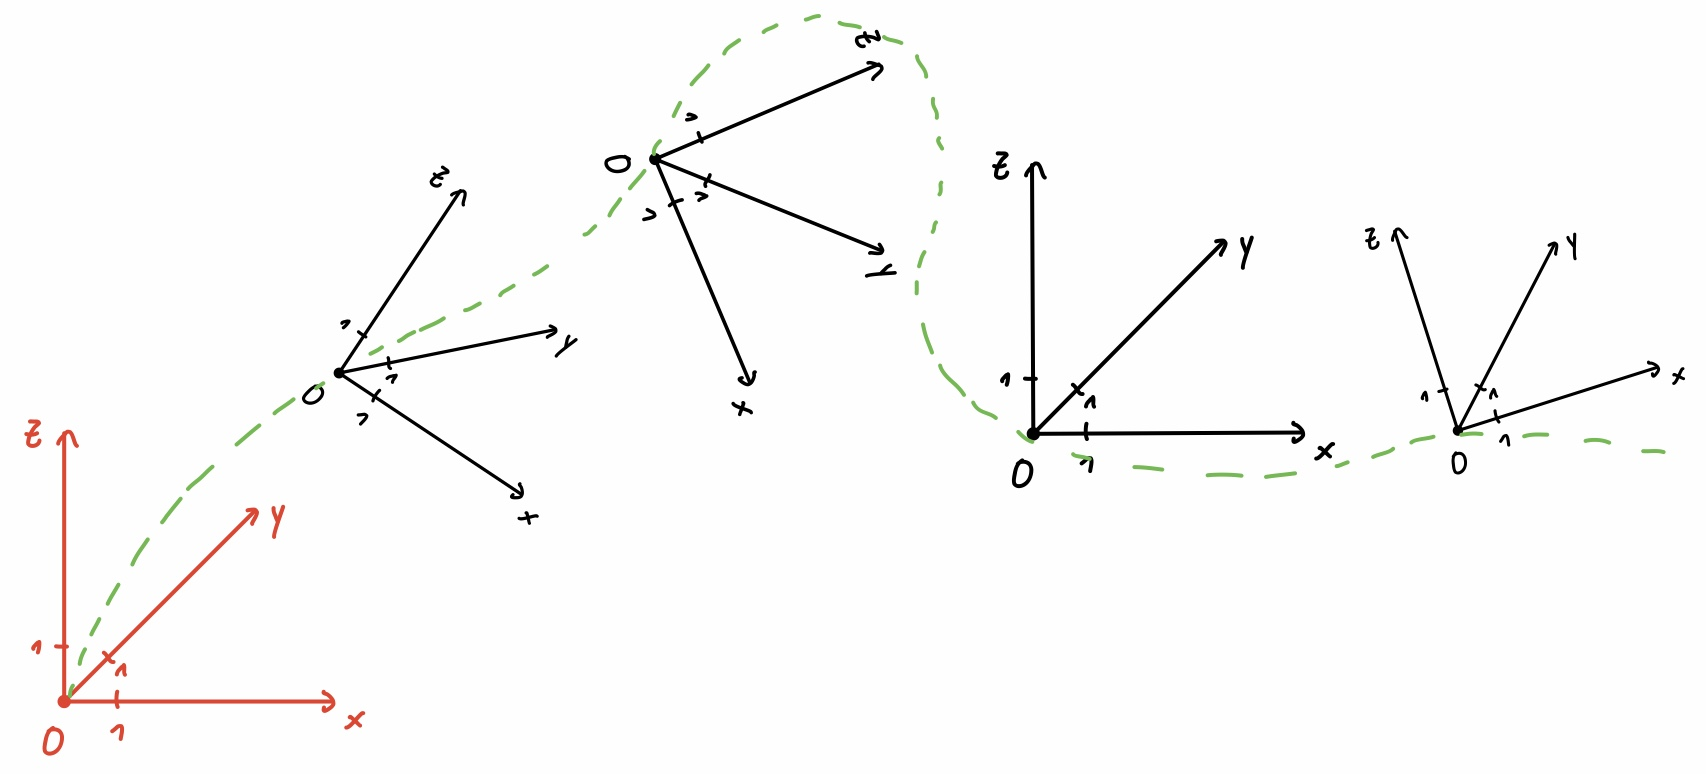
\includegraphics[width=0.75\textwidth]{koordinatnasistema}
\end{figure}

\noindent Označimo s $\underline{p}$ točko glede na fiksen koordinatni sistem $E^3$, s $\underline{\hat{p}}$ pa glede na $\hat{E}^3$. Potrebujemo koordinatno transformacijo
$$\hat{E}^3 \to E^3$$
$$\hat{p} \mapsto p$$

\noindent Z uporabo homogenih koordinat, lahko transformacijo zapišemo s pomočjo matrike

$$M =
\left[
\begin{tabular}{c | c c c}
$m_{0,0}$ & $0$ & $0$ & $0$ \\
\hline
$m_{1,0}$ & $m_{1,1}$ & $m_{1,2}$ & $m_{1,3}$ \\
$m_{2,0}$ & $m_{2,1}$ & $m_{2,2}$ & $m_{2,3}$ \\
$m_{3,0}$ & $m_{3,1}$ & $m_{3,2}$ & $m_{3,3}$ \\
\end{tabular}
\right],
$$

\noindent kjer velja $m_{0,0} \not=0$. Preslikavo v homogenih koordinatah lahko torej zapišemo kot:

$$\hat{p} \mapsto p = M \hat{p}$$

\noindent Vektorju $c = M (1,0,0,0)^T = (m_{0,0}, m_{1,0}, m_{2,3}, m_{3,0})^T$ zapisanemu v homogenih koordinatah pripada vektor $\underline{c} = (\frac{m_{1,0}}{m_{0,0}}, \frac{m_{2,0}}{m_{0,0}}, \frac{m_{3,0}}{m_{0,0}})^T$, zapisan v kartezičnih koordinatah. Ta vektor opisuje položaj koordinatnega izhodišča gibajočega se koordinatnega sistema $\hat{E}^3$ glede na koordinatni sistem $E^3$.

\noindent $3 \times 3$ matrika

$$\underline{R} =
\frac{1}{m_{0,0}}
\left[
\begin{tabular}{c c c}
$m_{1,1}$ & $m_{1,2}$ & $m_{1,3}$ \\
$m_{2,1}$ & $m_{2,2}$ & $m_{2,3}$ \\
$m_{3,1}$ & $m_{3,2}$ & $m_{3,3}$ \\
\end{tabular}
\right]
$$

\noindent opisuje orientacijo gibajočega se koordinatnega sistema $\hat{E}^3$. Pravimo ji \textbf{rotacijska matrika}.

%\noindent $\underline{c}$ predstavlja položaj izhodišča koordinatnega sistema $\hat{E}^3$ v koordinatni sistem $E^3$, $R$ pa je \textbf{rotacijska matrika}, ki opisuje rotacijo gibajočega se koordinatnega sistema. \\

\noindent Oglejmo si, kaj naredi matrika $M$ z vektorjem $[1,b_M,c_M,d_M]$:

$$M
\cdot
\left[
\begin{tabular}{c}
$1$ \\
$b_M$ \\
$c_M$ \\
$d_M$
\end{tabular}
\right]
=
\left[
\begin{tabular}{c}
$m_{0,0}$ \\
$m_{1,0}$ \\
$m_{2,0}$ \\
$m_{3,0}$ \\
\end{tabular}
\right]
+
\left[
\begin{tabular}{c c c}
$0$ & $0$ & $0$ \\
$m_{1,1} b_M$ & $m_{1,2} c_M$ & $m_{1,3} d_M$ \\
$m_{2,1} b_M$ & $m_{2,2} c_M$ & $m_{2,3} d_M$ \\
$m_{3,1} b_M$ & $m_{3,2} c_M$ & $m_{3,3} d_M$ \\
\end{tabular}
\right]
$$

\noindent Dobimo vektor v homogeni obliki, ki ima na prvi komponenti vrednost $m_{0,0}$, preostale tri komponente pa predstavlja vektor
$$\left[
\begin{tabular}{c}
$m_{1,0}$ \\
$m_{2,0}$ \\
$m_{3,0}$ \\
\end{tabular}
\right]
+
\left[
\begin{tabular}{c c c}
$m_{1,1}$ & $m_{1,2}$ & $m_{1,3}$ \\
$m_{2,1}$ & $m_{2,2}$ & $m_{2,3}$ \\
$m_{3,1}$ & $m_{3,2}$ & $m_{3,3}$ \\
\end{tabular}
\right]
\cdot
\left[
\begin{tabular}{c}
$b_M$ \\
$c_M$ \\
$d_M$
\end{tabular}
\right]
$$

Ker je to vektor v homogeni obliki in ker je prva komponenta neničelna ($m_{0,0} \not= 0$), je njemu prirejen vektor v kartezični obliki enak
$$\frac{1}{m_{0,0}}\left[
\begin{tabular}{c}
$m_{1,0}$ \\
$m_{2,0}$ \\
$m_{3,0}$ \\
\end{tabular}
\right]
+
\frac{1}{m_{0,0}}
\left[
\begin{tabular}{c c c}
$m_{1,1}$ & $m_{1,2}$ & $m_{1,3}$ \\
$m_{2,1}$ & $m_{2,2}$ & $m_{2,3}$ \\
$m_{3,1}$ & $m_{3,2}$ & $m_{3,3}$ \\
\end{tabular}
\right]
\cdot
\left[
\begin{tabular}{c}
$b_M$ \\
$c_M$ \\
$d_M$
\end{tabular}
\right],
$$

\noindent ki pa je enak vsoti $\underline{c} + R \cdot \underline{\hat{p}}$ 

\noindent Transformacijo $\underline{\hat{p}} \mapsto \underline{p}$ v kartezičnih koordinatah zapišemo kot:
$$\underline{p} = \underline{c} + R \underline{\hat{p}}$$

\subsection{Gibanje točk v času}

\noindent Kadar je $\underline{c} = \underline{c}(t)$ in $R=R(t)$, govorimo o gibanju togega telesa:
$$\hat{E}^3 \times I \to E^3$$
$$(\underline{\hat{p}},t) \mapsto \underline{c}(t) + R(t) \underline{\hat{p}} =: \underline{p}(t)$$
Krivulji $\underline{p}(t)$ pravimo \textbf{trajektorija} točke $\underline{\hat{p}}$ \\

\noindent Če je $\underline{c}(t) = (0,0,0)$, potem trajektorija poljubne točke $\underline{\hat{p}}$ leži na sferi z radijem $||\underline{\hat{p}}||$ in središčem v koordinatnem izhodišču fiksnega koordinatnega sistema $E^3$.
\noindent Rotacijski del gibanja $R(t)$ opisuje gibanje po enotski sferi, zato se imenuje tudi \textbf{sferični del gibanja togega telesa}. Problem je konstrukcija matrike $R$, ki mora biti ortogonalna. ($R R^T = R^T R = I$, $\det R = 1$). \\

\subsection{Opis rotacij s kvaternioni}
\noindent Pri opisovanju rotacij si lahko pomagamo s \textbf{kvaternioni}. Prostor kvaternionov $\H$ je $4$-dimenzionalni vektorski prostor s standardno bazo
$$ \underline{1} = (1, (0,0,0)^T) $$
$$ \underline{i} = (0,(1,0,0)^T) $$
$$ \underline{j} = (0,(0,1,0)^T) $$
$$ \underline{k} = (0,(0,0,1)^T) $$

\noindent Vsak kvaternion $\mathcal{A}$ lahko zapišemo kot:
$$\mathcal{A} = (a_0,\underline{a}),~ a_0 \in \R \text{ skalarni del },~ \underline{a} = (a_1,a_2,a_3)^T \text{ vektorski del}$$

\noindent Na kvaternionih sta definirana seštevanje in množenje kot:
$$\mathcal{A} + \mathcal{B} = (a_0,\underline{a}) +(b_0,\underline{b}) = (a_0 + b_0,\underline{a} + \underline{b})$$
$$\mathcal{A} \cdot \mathcal{B}  = (a_0 \cdot b_0 - \underline{a} \cdot \underline{b}, a_0 \underline{b} + b_0 \underline{a} + \underline{a} \times \underline{b})$$

\noindent Konjugirana vrednost kvaretniona $\mathcal{A} = (a_0,\underline{a})$ je definirana kot $\overline{\mathcal{A}} = (a_0, - \underline{a})$. S pomočjo konjugirane vrednosti nato definiramo tudi normo kvaterniona kot
$$|| \mathcal{A} || = \sqrt{\mathcal{A} \cdot \overline{\mathcal{A}}} = \sqrt{a_0^2 + a_1^2 + a_2^2 + a_3^2}$$

\begin{opomba}[Implementirane metode]
V implementaciji vektorski del kvaterniona $a$ pridobimo s funkcijo $quat\_vec(a)$, sklararni del pa kar z ukazom $a(1)$. Kvaterniona $a$ in $b$ seštejemo z ukazom $a+b$, njun produkt pa kličemo s funkcjio $quatmultiply(a,b)$. Konjugirano vrednost kvaterniona $a$ pridobimo s klicom funkcije $conj\_quat(a)$. Za kvaternion $a$ normo izračunamo z ukazom $sum(a.^2)$.
\end{opomba}

\begin{definicija}
\label{definicijarotacije}
Preslikava $\chi : \H \backslash \{0\} \to SO_3$ oblike

$$Q  \mapsto \frac{1}{q_0^2 + q_1^2 + q_2^2 + q_3^2}
\left[
\begin{tabular}{c c c}
$q_0^2 + q_1^2 - q_2^2 - q_3^2$ & $2(q_1 q_2 - q_0 q_3)$ & $2(q_1 q_3 + q_0 q_2)$ \\
& & \\
$2(q_1 q_2 + q_0 q_3)$ & $q_0^2 - q_1^2 + q_2^2 - q_3^2$ & $2(q_2 q_3 - q_0 q_1)$ \\
& & \\
$2(q_1 q_3 - q_0 q_2)$ & $2(q_2 q_3 + q_0 q_2)$ & $q_0^2 - q_1^2 - q_2^2 + q_3^2$
\end{tabular}
\right]
$$

$$ Q = (q_0,(q_1,q_2,q_3)^T)$$
\\
se imenuje \textbf{kinematična preslikava}.
\end{definicija}

\noindent Matika $\chi(Q)$ je rotacijska matrika. Velja pa tudi obratno. Vsako rotacijsko matriko $R$ lahko zapišemo v zgornji obliki, to je, lahko jo preslikamo v dva \textbf{antipodna kvaterniona} oblike
$$\pm Q = \pm(q_0,(q_1,q_2,q_3)^T),$$
$$q_0^2 + q_1^2 + q_2^2 + q_3^2 = 1$$

\noindent \textbf{Kinematična preslikava} poda korespondenco med 3D rotacijami in parom antipodnih točk na 4D enotski sferi $S^3 \subseteq R^4$. \\

\noindent Ker velja $q_0^2 + q_1^2 + q_2^2 + q_3^2 = 1$, so vrednosti $|q_i|;~ i=0,1,2,3$ na zaprtem interalu med $0$ in $1$. Vrednost $q_0$ in vektor $(q_1,q_2,q_3)^T$ lahko zato zapišemo v obliki:

$$q_0 = \cos(\frac{\phi}{2})$$

in

$$\left[
\begin{tabular}{c}
$q_1$ \\
$q_2$ \\
$q_3$
\end{tabular}
\right]
=
\sin(\frac{\phi}{2}) \cdot \vec{r}; ~ \vec{r} \text{ enotski vektor}
$$

\noindent Če kvaternion $Q$ zapišemo v tej obliki, ima rotacija, prirejena temu kvaternionu lepo geometrijsko interpretacijo. Predstavlja namreč rotacijo za kot $\phi$ okrog osi $\vec{r}$. \\


\begin{opomba}[Implementirane metode] V implementaciji rotacijsko matriko, prirejeno kvaternionu $a$ generiramo s funkcijo $quat\_rot\_mat(a)$. Če imamo podan kot $\phi$ in enotski vektor $r$, nam funkcija $kot\_v\_kvat(\phi,r)$ poda pripadajoč kvaternion.

\end{opomba}

\noindent Ker lahko vsako rotacijo zapišemo v tej obliki, lahko tako zapišemo tudi rotacijo iz poglavja \ref{zvezaFiksnikoor-Gibajockoor}. Če imamo podano preslikavo $M$, poiščimo, kako za to preslikavo definiramo kvaternion $Q$. Priemerjajmo matriki $\R$ in poglavja \ref{zvezaFiksnikoor-Gibajockoor} in $\R$, zapisanega s kvaternioni.

\begin{align*}
m_{0,0} + m_{1,1} + m_{1,2} + m_{3,3} &= 4 q_0^2 \\
m_{3,2} - m_{2,3} = 2 \cdot (q_2 q_3 - q_0 q_1) - 2 \cdot (q_2 q_3 + q_0 q_1) &= 4 q_0 q_1 \\
m_{1,3} - m_{3,1} = 2 \cdot (q_1 q_3 + q_0 q_2) - 2 \cdot (q_1 q_3 + q_0 q_2) &= 4 q_0 q_2 \\
m_{2,1} - m_{1,2} = 2 \cdot (q_1 q_2 + q_0 q_4) - 2 \cdot (q_1 q_2 + q_0 q_4) &= 4 q_0 q_3 \\
& \\
m_{3,2} - m_{2,3} & = 4 q_0 q_1 \\
m_{0,0} + m_{1,1} - m_{1,2} - m_{3,3} &= 4 q_1^2 \\
m_{2,1} + m_{1,2} &= 4 q_1 q_2 \\
m_{1,3} + m_{3,1} &= 4 q_1 q_3 \\
& \\
m_{1,3} - m_{3,1} &= 4 q_0 q_2 \\
m_{2,1} + m_{1,2} &= 4 q_1 q_2 \\
m_{0,0} - m_{1,1} + m_{1,2} - m_{3,3} &= 4 q_2^2 \\
m_{3,2} + m_{2,3} &= 4 q_2 q_3 \\
& \\
m_{2,1} - m_{1,2} &= 4 q_0 q_3 \\
m_{1,3} + m_{3,1} &= 4 q_1 q_3 \\
m_{3,2} + m_{2,3} &= 4 q_2 q_3 \\
m_{0,0} - m_{1,1} - m_{1,2} + m_{3,3} &= 4 q_0^2 \\
\end{align*}

\noindent Opazimo, da v vsakem sklopu razmerja med vrednostmi enaka
$$ q_0 : q_1 : q_2 : q_3 $$

\noindent Ker $q_0,q_1,q_2,q_3$ niso hkrati enaki $0$, bo vsaj eno izmed zgornjih razmerij različno od $0 : 0 : 0 : 0$. Tisto razmerje nato uporabimo kot razmerje $ q_0 : q_1 : q_2 : q_3 $. Skupaj z enakostjo $q_0^2 + q_1^2 + q_2^2 + q_3^2 = 1$ nato izračunamo kvaternion $Q=(q_0,q_1,q_2,q_3)^T$ (bolj natančno sta v množici rešitev dva antipodna kvaterniona).
\subsection{Bezierjeve krivulje}
\noindent Z uporabo kinematične preslikave lahko za konstrukcijo sferičnih gibanj uporabimo Bezierjeve krivulje. Izberemo kontrolne kvaternione $Q_0,Q_1,\dots,Q_n$.
$$Q(t) = \sum\limits_{i=0}^{n} Q_i B_i^n(t)$$
\noindent Bezierjeva krivulja $Q(t)$ v času $t$ opiše kvaternion, ki mu priredimo rotacijo $R(t)$:
$$\chi(Q(t)) = R(t)$$

\noindent Rotacija, ki je določena z Bezierjevo krivuljo $Q(t) = \sum\limits_{i=0}^{n} Q_i B_i^n(t)$ stopnje $n$, je sferično razionalno gibanje stopnje $2n$. \\

\noindent Gibanje koordinatnega izhodišča zapišemo v obliki
$$\underline{c}(t) = \frac{w(t)}{||Q(t)||^2};~ w(t) := (w_1(t), w_2(t),w_3(t)).$$

\begin{opomba}
Za računanje Bezierjeve krivulje rotacije uporabimo funkciji $sbezier$ in $sdecasteljau$, za gibanje koordinatnega izhodišča pa $bezier$ in $decasteljau$.
\end{opomba}

\newpage

\section{Implementacija}

\subsection{Kvaternioni}
Ker si pri opisovanju rotacij pomagamo s kvaternioni, sva na kvaternionih definirala naslednje funkcije:

%\begin{lstlisting}[caption = {\color{red} array2quat}]
%function Q = array2quat(a, b, c, d)
%%ARRAY2QUAT prejme 4 parametre, ki jih pretvori v kvaternion (vektorsko obliko)
%%input:
%%a, b, c, d     komponente   
%%output:
%%Q              kvaternion
%
%Q = [a, b, c, d];
%end
%\end{lstlisting}

\vspace{1cm}
\textbf{Vektorski del kvaterniona:}\\
Input:
\begin{itemize}
\item kvaternion $Q$ oblike $[q_0,q_1,q_2,q_3]$
\end{itemize}
Output:
\begin{itemize}
\item vektorski del $v$ ($q_1,q_2,q_3$) kvaterniona $Q$
\end{itemize}

\begin{lstlisting}[caption = {quat\_vec}]
function v = quat_vec(Q)

v = [Q(2) Q(3) Q(4)];
end
\end{lstlisting}


\vspace{1cm}
\textbf{Množenje kvaternionov:}\\
Input:
\begin{itemize}
\item kvaternion $a$ oblike $[a_1,a_2,a_3,a_4]$
\item kvaternion $b$ oblike $[b_1,b_2,b_3,b_4]$
\end{itemize}
Output:
\begin{itemize}
\item kvaternion $c = a \cdot b$
\end{itemize}

\begin{lstlisting}[caption = {quatmultiply}]
function c = quatmultiply(a,b)

c = zeros(1,4);
a_s = a(1);
b_s = b(1);
a_v = quat_vec(a);
b_v = quat_vec(b);
c(1) = a_s * b_s - a_v * b_v';
c_v = a_s * b_v + b_s * a_v + cross(a_v,b_v);
c(2) = c_v(1);
c(3) = c_v(2);
c(4) = c_v(3);
end
\end{lstlisting}

\textbf{Konjugirana vrednost kvaterniona:}\\
Input:
\begin{itemize}
\item kvaternion $q$ oblike $[q_1,q_2,q_3,q_4]$
\end{itemize}
Output:
\begin{itemize}
\item kvaternion $Q = \overline{q}$
\end{itemize}

\begin{lstlisting}[caption = {conj\_quat}]
function Q = conj_quat(q)

Q = [q(1), -q(2:4)];
end
\end{lstlisting}


\vspace{0.5cm}
\textbf{Potenca kvaterniona $q$:}\\
Input:
\begin{itemize}
\item kvaternion $q$ oblike $[q_1,q_2,q_3,q_4]$
\item eksponent $t$
\end{itemize}
Output:
\begin{itemize}
\item $q^t$
\end{itemize}
\begin{lstlisting}[caption = {quat\_exp}]
function e = quat_exp(q, t)

if t==-1
    e = conj_quat(q)/norm(q);
else
    a = q(1);
    v = quat_vec(q);
    theta = acos(a/norm(q));
    n = v/norm(v);
    e = norm(q)^t*[cos(t*theta), n*sin(t*theta)];
end
\end{lstlisting}

\vspace{1cm}

\textbf{Rotacijska matrika:}\\
Input:
\begin{itemize}
\item kvaternion $q$ oblike $[q_1,q_2,q_3,q_4]$
\end{itemize}
Output: 
\begin{itemize}
\item rotacijska matrika $H$ za sfericno gibanje
\end{itemize}

\begin{lstlisting}[caption = {quat\_rot\_mat}]
function H = quat_rot_mat(Q)

H = zeros(3,3);
h = sum(Q.^2);

if h == 0
    H = eye(3,3);
else
    H(1,1) = Q(1)^2+Q(2)^2 - Q(3)^2 - Q(4)^2;
    H(1,2) = 2*(Q(2)*Q(3) - Q(1)*Q(4));
    H(1,3) = 2*(Q(2)*Q(4) + Q(1)*Q(3));

    H(2,1) = 2*(Q(2)*Q(3) + Q(1)*Q(4));
    H(2,2) = Q(1)^2 - Q(2)^2 + Q(3)^2 - Q(4)^2;
    H(2,3) = 2*(Q(3)*Q(4) - Q(1)*Q(2));

    H(3,1) = 2*(Q(2)*Q(4) - Q(1)*Q(3));
    H(3,2) = 2*(Q(3)*Q(4) + Q(1)*Q(2));
    H(3,3) = Q(1)^2 - Q(2)^2 - Q(3)^2 + Q(4)^2;

    H = 1/h.*H;  
end
end
\end{lstlisting}

\vspace{1cm}
\textbf{Kvaternion glede na rotacijo za kot $\phi$ okrog osti $e$:}\\
Input:
\begin{itemize}
\item kot $fi$
\item vektor osi $e$
\end{itemize}
Output:
\begin{itemize}
\item kvaternion $Q$
\end{itemize}

\begin{lstlisting}[caption = {kot\_v\_kvat}]
function r = kot_v_kvat(fi, e)

e = e/norm(e);
r = [cos(fi/2) sin(fi/2)*e(1) sin(fi/2)*e(2) sin(fi/2)*e(3)];
end
\end{lstlisting}

\newpage

\textbf{Rotacija vektorja okrog koordinatnih osi:}\\
Input:
\begin{itemize}
\item vektor $vec$
\item koti $kot\_x$, $kot\_y$, $kot\_z$ rotacije okrog $x$,$y$,$z$ osi
\end{itemize}
Output:
\begin{itemize}
\item zarotiran vektor $v$
\end{itemize}

\begin{lstlisting}[caption = {rot\_vek\_za\_kot}]
function v = rot_vek_za_kot(vec, kot_x,kot_y,kot_z)

q = angle2quat(kot_x, kot_y, kot_z);
v = quatmultiply(q, quatmultiply([0 vec], conj_quat(q)));
end
\end{lstlisting}

\newpage

\subsection{Bezierjeve krivulje}

\textbf{Bezier:}\\
Input:
\begin{itemize}
\item matrika $B$ velikosti $(n+1) \times d$, ki predstavlja kontrolne točke Bezierjeve krivulje
\item seznam parametrov $t$ dolzine $k$, pri katerih računamo vrednost Bezierjeve krivulje
\end{itemize}
Output:
\begin{itemize}
\item matrika $b$, ki predstavlja točke na Bezierjevi krivulji pri parametrih iz $t$
\end{itemize}

\begin{lstlisting}[caption = {bezier}]
function b = bezier (B,t)

[n,d] = size(B);
k = length(t);
b = zeros(k,d);

for i=1:k
    for j=1:d
        D = decasteljau(B(:,j)',t(i));
        b(i,j) = D(1,n);
    end
end
\end{lstlisting}

\vspace{1cm}
\textbf{Decasteljau:}\\
Input:
\begin{itemize}
\item seznam koordinat $b$ kontrolnih točk Bezierjeve krivulje stopnje $n$
\item parameter $t$, pri katerem računamo koordinato Bezierjeve krivulje
\end{itemize}
Output:
\begin{itemize}
\item Casteljaujeva shema $D$
\end{itemize}

\begin{lstlisting}[caption = {decasteljau}]
function D = decasteljau (b,t) 

n = length(b);
D = [b', NaN(n,n-1)];

for r=1:n
    for i=0:n-r-1
        D(i+1,r+1) = (1-t)*D(i+1,r) + t*D(i+2,r);
    end
end
\end{lstlisting}

\newpage

\textbf{sBezier:}\\
Input:
\begin{itemize}
\item matrika $Q$ velikosti $(n+1) \times d$, ki predstavlja kontrolne točke Bezierjeve krivulje
\item seznam parametrov $t$ dolzine $k$, pri katerih računamo vrednost Bezierjeve krivulje
\end{itemize}
Output:
\begin{itemize}
\item matrika $b$, ki predstavlja točke na Bezierjevi krivulji pri parametrih iz $t$
\end{itemize}

\begin{lstlisting}[caption = {sbezier}]
function b = sbezier(Q,t)
k = length(t);

b = cell(k,1);

for K = 1:k
    decast = sdecasteljau(Q,t(K));
    b{K} = decast(1,end);
end
b;
\end{lstlisting}

\vspace{0.5cm}
\textbf{sDecasteljau:}\\
Input:
\begin{itemize}
\item seznam koordinat $Q$ kontrolnih točk Bezierjeve krivulje stopnje $n$
\item parameter $t$, pri katerem računamo koordinato Bezierjeve krivulje
\end{itemize}
Output:
\begin{itemize}
\item Casteljaujeva shema $D$
\end{itemize}

\begin{lstlisting}[caption = {sdecasteljau}]
function D = sdecasteljau(Q,t)

[n,m] = size(Q);
n = n-1;
D = cell(n+1, n+1);
for i = 1:(n+1)
    D{i,1} = Q(i,:);
end
for j=2:(n+1)
    for i=1:(n+2-j)
        D{i,j} = slerp(D{i,j-1},D{i+1,j-1},t);
    end
end
end
\end{lstlisting}

\textbf{Matrika iz celice:}\\
Input:
\begin{itemize}
\item celica $Q$
\end{itemize}
Output:
\begin{itemize}
\item matrika $Q$
\end{itemize}

\begin{lstlisting}[caption = {polepsaj\_sbezier}]
function mat_Q = polepsaj_sbezier(Q)

n = length(Q);
mat_Q = zeros(n,4);
for i = 1:n
    mat_Q(i,:) = Q{i}{1};
end
end
\end{lstlisting}

\vspace{1cm}
\textbf{Translacija izhodišča:}\\
Input:
\begin{itemize}
\item translacijska funkcija izhodišča $w$, računana na $t$ ($n \times 3$ matrika)
\item sferična rotacijska Bezierjeva krivulja, računana na t ($n \times 4$ matrika)
\item seznam parametrov $t$ dolžine $n$, pri katerih računamo funkcijo.
\end{itemize}
Output:
\begin{itemize}
\item normirana translacija ($n \times 3$ matrika)
\end{itemize}

\begin{lstlisting}[caption = {translacija}]
function c = translacija(w, Q, t)

n = length(t);
c = zeros(n,3);

for i = 1:n
    nQt = norm(Q(i,:))^2;
    c(i,:) = w(i,:)/nQt;
end
end
\end{lstlisting}

\newpage

\textbf{Celotno gibanje togega telesa:}\\
Input:
\begin{itemize}
\item matrika kontrolnih kvaternionov $Q$ za sferične rotacije
\item matrika kontrolnih točk za Bezierjevo krivuljo gibanja izhodišča
\item seznam parametrov $t$, pri katerih opazujemo gibanje
\end{itemize}
Output:
\begin{itemize}
\item matrika kvaternionov $mat_Q$, ki določajo sferične rotacije
\item Bezierjeva krivulja $w$, ki določa gibanje koordinatnega izhodišča
\item normirana translacijska funkcija $c$
\end{itemize}

\begin{lstlisting}[caption = {izracunaj\_vse}]
function [mat_Q,w,c] = izracunaj_vse(Q, B, t)

mat_Q = polepsaj_sbezier(sbezier(Q,t));
w = bezier(B,t);
c = translacija(w,mat_Q, t);
end
\end{lstlisting}

\newpage

\subsection{Kocka}

\textbf{Oglišča kocke z diagonalo $d$:}\\
Input:
\begin{itemize}
\item krajišči diagonale $T0$ in $T1$ $(d=T0 T1)$
\end{itemize}
Output:
\begin{itemize}
\item koorinate oglišč kocke
\end{itemize}

\begin{lstlisting}[caption = {kocka}]
function oglisca = kocka(T0, T1)

a = [T1(1) - T0(1) 0 0];
b = [0 T1(2) - T0(2) 0];
c = [0 0 T1(3) - T0(3)];
oglisca = [T0; T0+b; T0+a+b; T0+a; T0+c; T0+c+b; T0+a+b+c; T0+a+c];
end
\end{lstlisting}

\vspace{1cm}
\textbf{Kocka s stranicami in izhodiščem:}\\
Input:
\begin{itemize}
\item vektorji stranic $X$,$Y$,$Z$
\item izhodišče $T0$
\end{itemize}
Output:
\begin{itemize}
\item vsa oglišča kocke, ki se začne v T0
\end{itemize}

\begin{lstlisting}[caption = {kocka\_vek}]
function oglisca = kocka_vek(X, Y, Z, T0)

oglisca = [T0; T0+Y; T0+X+Y; T0+X; T0+Z; T0+Z+Y; T0+X+Y+Z; T0+X+Z];
end
\end{lstlisting}

\vspace{1cm}
\textbf{Slika kocke:}\\
Input:
\begin{itemize}
\item koordinate oglišč $K$
\item barva $barva$
\end{itemize}
Output:
\begin{itemize}
\item slika kocke
\end{itemize}

\begin{lstlisting}[caption = {\color{red} risi\_kocko}]
function risi_kocko(K, barva)

ploskve = [1 2 3 4; 2 6 7 3; 4 3 7 8; 1 5 8 4; 1 2 6 5; 5 6 7 8]; 
patch('Vertices', K, 'Faces', ploskve, 'FaceColor', barva);
end
\end{lstlisting}

\vspace{0.5cm}
\textbf{Rotacija kocke:}\\
Input:
\begin{itemize}
\item kocka $K0$
\item koti $kot\_x$, $kot\_y$, $kot\_z$
\end{itemize}
Output:
\begin{itemize}
\item $K1$ - zarotirana kocka $K0$ za podane kote
\end{itemize}

\begin{lstlisting}[caption = {rotiraj\_kocko}]
function K1 = rotiraj_kocko(K0, kot_x, kot_y, kot_z)

K1 = zeros(size(K0));
for i = 1:8
    K1(i,:) = quat_vec(rot_vek_za_kot(K0(i,:), kot_x, kot_y, kot_z));
end
end
\end{lstlisting}

\vspace{0.5cm}
\textbf{Rotacija kocke:}\\
Input:
\begin{itemize}
\item kvaternion $Q$
\item vektorji stranic kocke $x$,$y$ in $z$
\end{itemize}
Output:
\begin{itemize}
\item Oglišča zarotirane kocke z enim ogliščem v $[0,0,0]$
\end{itemize}

\begin{lstlisting}[caption = {rotirana\_kocka}]
function [K0, x0, y0, z0] = rotirana_kocka(x,y,z,Q)

H = quat_rot_mat(Q);
x0 = (H*x')';
y0 = (H*y')'; 
z0 = (H*z')';
K0 = kocka_vek(x0,y0,z0, [0 0 0]);

end
\end{lstlisting}

\newpage


\textbf{Gibanje kocke:}\\
Input:
\begin{itemize}
\item vektorji $x$,$y$ in $z$, i določajo začetno kocko.
\item izhodišče kocke $T0$
\item matrika $B$ kontrolnih kvaternionov
\item translacijska funkcija $c$ izhodišča gibajočega se koordinatnega sistema
\item barve $zac\_barva$, $vmes_barva$, $kon_barva$ kontrolnih kvadrov
\item argument $pavza$, ki pove, ali naj slika poteka v obliki gibanja
\end{itemize}
Output:
\begin{itemize}
\item slika gibanja kvadra
\end{itemize}

\begin{lstlisting}[caption = {\color{red} plot\_kontrolne\_kocke}]
function  plot_kontrolne_kocke(x0,y0,z0,T0, B,c, zac_barva, vmes_barva, kon_barva, pavza)

for i = 1:size(B,1)
    if pavza
        pause
    end
    switch i
        case 1
            barva = zac_barva;
        case size(B,1)
            barva = kon_barva;
        otherwise
            barva = vmes_barva;
    end
    Q = B(i,:);
    H = quat_rot_mat(Q);
    x = (H*x0')';
    y = (H*y0')';
    z = (H*z0')';
    T = T0+c(i,:);
    risi_kocko(kocka_vek(x, y, z, T),barva);
end
\end{lstlisting}

\newpage
\subsection{Razvrsti}

\textbf{:}\\
Input:
\begin{itemize}
\item 
\end{itemize}
Output:
\begin{itemize}
\item 
\end{itemize}

\begin{lstlisting}[caption = {\color{red} plot\_tirnice}]
function plot_tirnice(P, c)
%input:
% P                 premaknjeni vektorji kvadra
% c                 translacijska funkcija
%ouput:
% narise "tirnice", po katerih se premikajo oglisca kvadra

n = size(c, 1);

%en vektor
V_x = zeros(n,3);
V_y = zeros(n,3);
V_z = zeros(n,3);
V_xy = zeros(n,3);
V_zy = zeros(n,3);
V_xz = zeros(n,3);
V = zeros(n,3);


for i = 1:n
    Pi = P{i};
    V_x(i,:) = Pi(1,:);
    V_y(i,:) = Pi(2,:);
    V_z(i,:) = Pi(3,:); 
end

% dva vektorja
V_xy = V_x + V_y + c;
V_zy = V_z + V_y + c;
V_xz = V_x + V_z + c;

% vsi
V = V_x + V_y + V_z + c;

V_x = V_x + c;
V_y = V_y + c;
V_z = V_z + c;


plot3(V_x(:,1), V_x(:,2), V_x(:,3),...
    V_y(:,1), V_y(:,2), V_y(:,3),...
    V_z(:,1), V_z(:,2), V_z(:,3),...
    V_xy(:,1), V_xy(:,2), V_xy(:,3),...
    V_zy(:,1), V_zy(:,2), V_zy(:,3),...
    V_xz(:,1), V_xz(:,2), V_xz(:,3),...
    V(:,1), V(:,2), V(:,3),...
    c(:,1), c(:,2), c(:,3),...
    'LineWidth',1.5)


end
\end{lstlisting}


\begin{lstlisting}[caption = {\color{green} slerp}]
function Q = slerp(Q1, Q2, t)
%input:
% Q1, Q2            kvaterniona
% t                 parameter v [0,1]
%output:
% Q                 rezultat slerp-a med Q1 in Q2 na mestu t
%To je sfericna linearna interpolacija, ki naj bi zamenjala
%navadno v de Casteljauju.
% https://en.wikipedia.org/wiki/Slerp

if t == 0
    Q = Q1;
else
    if t == 1
        Q = Q2;
    else
%         q = quatmultiply(Q1,Q2);
%         if q(1) <= 0 
%             display('dolga pot')
%             display(q)
%             [r1,r2,r3] = quat2angle(q)
%             %Q1 = -Q1; %tako naj bi izbrala krajso pot, se mi zdi 
%         end
        Q = quatmultiply(Q1, quat_exp(quatmultiply(quat_exp(Q1,-1),Q2),t));
    end
end
end
\end{lstlisting}

\textbf{:}\\
Input:
\begin{itemize}
\item 
\end{itemize}
Output:
\begin{itemize}
\item 
\end{itemize}

\begin{lstlisting}[caption = {\color{red} narisi\_vse}]
function narisi_vse(x0,y0,z0,T0, mat_Q,c, t, osi, prehod,tirnice,robovi)
%Tole bo narisalo vse
%input:
% x0,y0,z0                  stranice kvadra
% T0                        izhodisce kvadra
% mat_Q                     matrika sfericnih rotacij
% c                         matrika normirane translacijske funkcije
% t                         parametri, pri katerih racunamo
% osi                       dolzine osi
% prehod, tirnice, robovi   1 ali 0, kaj hocemo risati
n = length(t);

H = cell(n,1);
P = cell(n,1);
hold on
axis equal
axis([-osi osi -osi osi -osi osi])

% Rise prehajanje kvadrov

for i = 1:n
    H{i} = quat_rot_mat(mat_Q(i,:));
    x = (H{i}*x0')';
    y = (H{i}*y0')';
    z = (H{i}*z0')';
    P{i} = [x;y;z];
    if prehod
        if (mod(i, 1) == 0 || i == 1)
            risi_kocko(kocka_vek(x, y, z, c(i,:)), [(n-i)/n, 0, i/n]);
        end
    end
end

% Rise tirnice, po katerih se premikajo oglisca kvadra
if tirnice
    plot_tirnice(P,c)
    plot3(c(:,1), c(:,2), c(:,3),'LineWidth', 2, 'Color', 'k')
end
% Narise izracunano prvo in zadnje stanje
if robovi
    H = quat_rot_mat(mat_Q(end,:));
    x = (H*x0')';
    y = (H*y0')';
    z = (H*z0')';
    T = T0+c(end,:);
    risi_kocko(kocka_vek(x, y, z, T),'g');
    H = quat_rot_mat(mat_Q(1,:));
    x = (H*x0')';
    y = (H*y0')';
    z = (H*z0')';
    T = T0+c(1,:);
    risi_kocko(kocka_vek(x, y, z, T),'y');
end
end
\end{lstlisting}

\end{document}
